\begin{figure}
	\tikzsetnextfilename{plot_mws_int}
	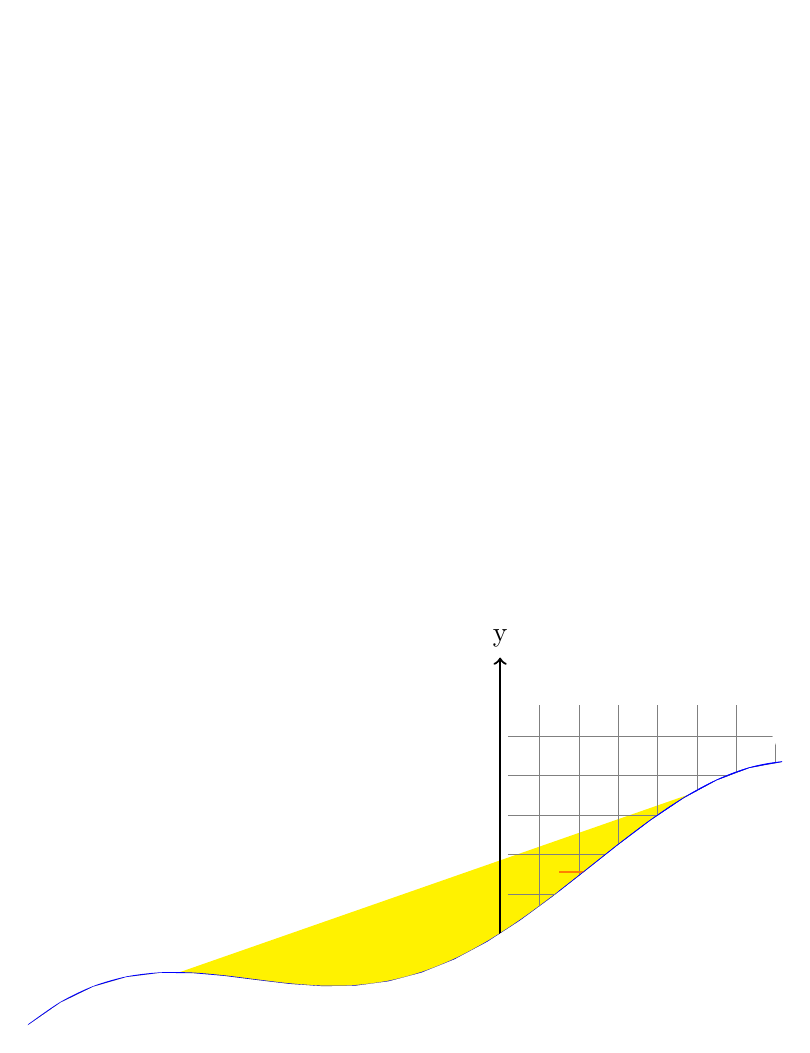
\begin{tikzpicture}
		\path[clip] plot (\x,{(2*sin(0.5*\x r)+2)*(1/6)*\x}) -- (1,12);
		\filldraw[color=blue,fill=yellow] plot[smooth] (\x,{(2*sin(0.5*\x r)+2)*(1/6)*\x});
		\draw[very thin, gray, step = 0.5] (1.1,-0.4) grid (12.4,3.4);
		\draw[->, thick, black] (1,-0.5) -- (12,-0.5) node[right]{x};
		\draw[->, thick, black] (1,-0.5) --(1,4) node[above]{y};
		\draw[thick, orange, domain= 1.75:12.25] plot(\x, 1.28);
		\draw[blue, domain = 1.75: 12,samples = 1000] 
			plot (\x, {(2*sin(0.5*\x r)+2)*(1/6)*\x});
		\draw[fill = black](7.34,1.28) circle (1pt) node[above]{c};
	%
	\end{tikzpicture}
\end{figure}
